\subsection{The Cauchy problem = initial value problem}
\begin{frame}{The Cauchy problem = initial value problem}

  \begin{block}{Definition on a half-plane}
  Szukamy u(x,t):
\begin{itemize}    
\item określonej
\item ciągłej
\end{itemize}
	 dla:
   
$-\infty < x < \infty, t \ge 0 $ \\
spełniającej (\ref{etykieta}) dla \\
$-\infty < x <\infty, t > 0 $


oraz spełniającej warunki początkowe:
\begin{equation}u(x,0) = f_1(x), -\infty < x < \infty\end{equation}
\begin{equation}u_t(x,0) = f_2(x), -\infty < x < \infty\end{equation}
$f_1(x), f_2(x) $ -- zadane funkcje
\end{block}
\end{frame}

\begin{frame}
  \centerline{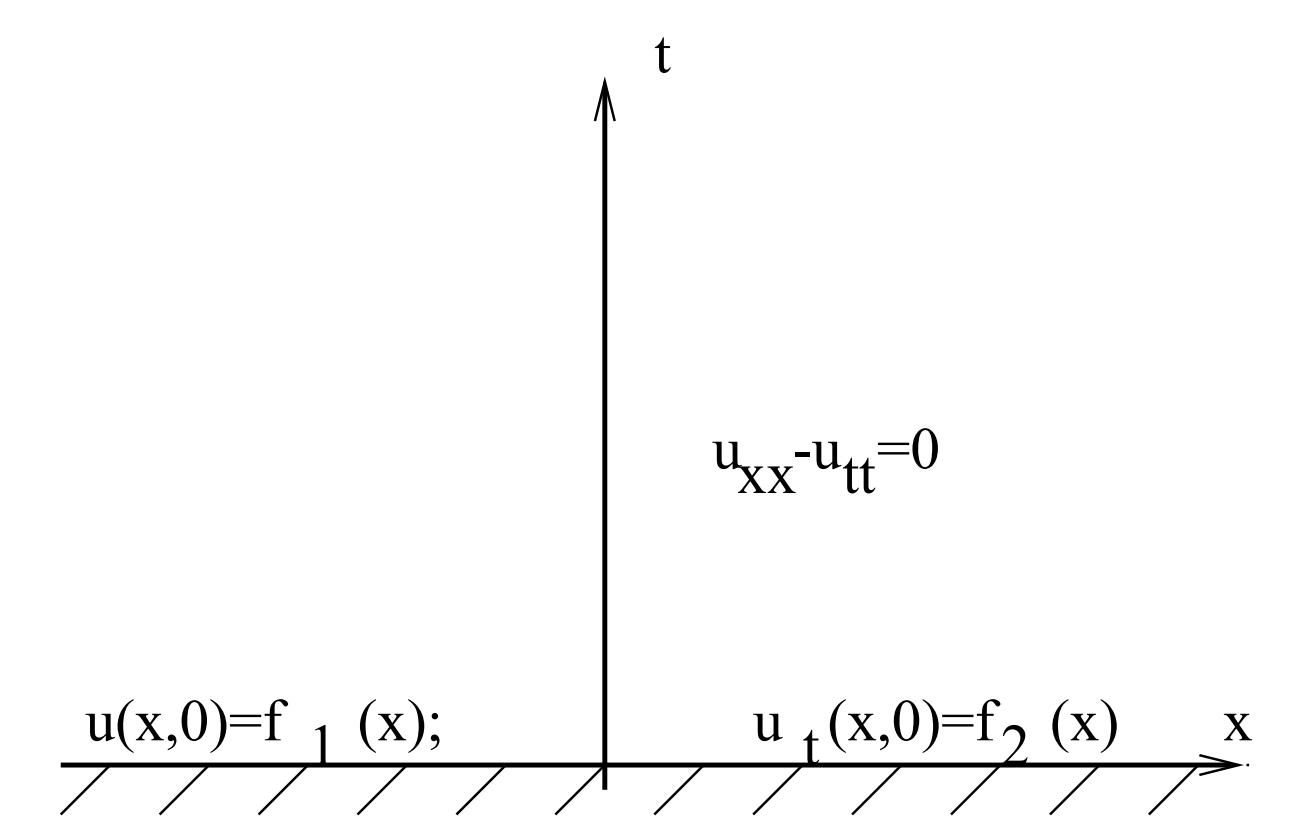
\includegraphics[height = 0.85 \textheight]{img/23/cauchy}}
\end{frame}